\documentclass[a4paper]{article}
\usepackage[document]{ragged2e}
\usepackage{fontspec}
\usepackage{geometry}
\usepackage{graphicx}
\usepackage{url}
\geometry{left=2cm}
\geometry{right=2cm}
\geometry{top=2cm}
\geometry{bottom=2cm}
\setmainfont{Liberation Serif}
\setmonofont[Scale=0.8]{Hack}
\sloppy

\graphicspath{ {./pics/} }

\begin{document}
  \fontsize{14}{16}\selectfont

  \begin{titlepage}
    \begin{minipage}{0.2\textwidth}
      
\includegraphics[scale=0.4]{logo}
    \end{minipage}
    \begin{minipage}{0.7\textwidth}\centering
      \fontsize{10}{12}\selectfont
      \textbf{
        Федеральное государственное бюджетное образовательное учреждение \\
        высшего профессионального образования \\
        «Московский государственный технический университет имени Н.Э. Баумана» \\
        (МГТУ им. Н.Э. Баумана)
      }
    \end{minipage}

    \vspace{5cm}
    \centering
    \textbf{
      Рубежный контроль 1 \\
      по курсу «Технологии машинного обучения» \\
    }

    \vspace{5cm}
    \begin{flushright}
    Выполнил \\
    студент группы ИУ5-64 \\
    XXX \\
    Вариант 7
    \end{flushright}
    \vspace*{\fill}
    Москва, 2021
  \end{titlepage}

  \section*{Задание}
  \begin{center}
    \begin{tabular}{|c|c|c|}
      \hline
      Номер варианта & Номер задачи & Номер набора данных, указанного в задаче \\
      \hline
      7 & 1 & 7 \\
      \hline
    \end{tabular}
  \end{center}

  Для заданного набора данных проведите корреляционный анализ.
  В случае наличия пропусков в данных удалите строки или колонки, содержащие пропуски.
  Сделайте выводы о возможности построения моделей машинного обучения и о возможном вкладе признаков в модель. \\
  \textbf{Дополнительное требование:} для произвольной колонки данных построить график "Скрипичная диаграмма (violin plot)".

  \section*{Ход работы}
  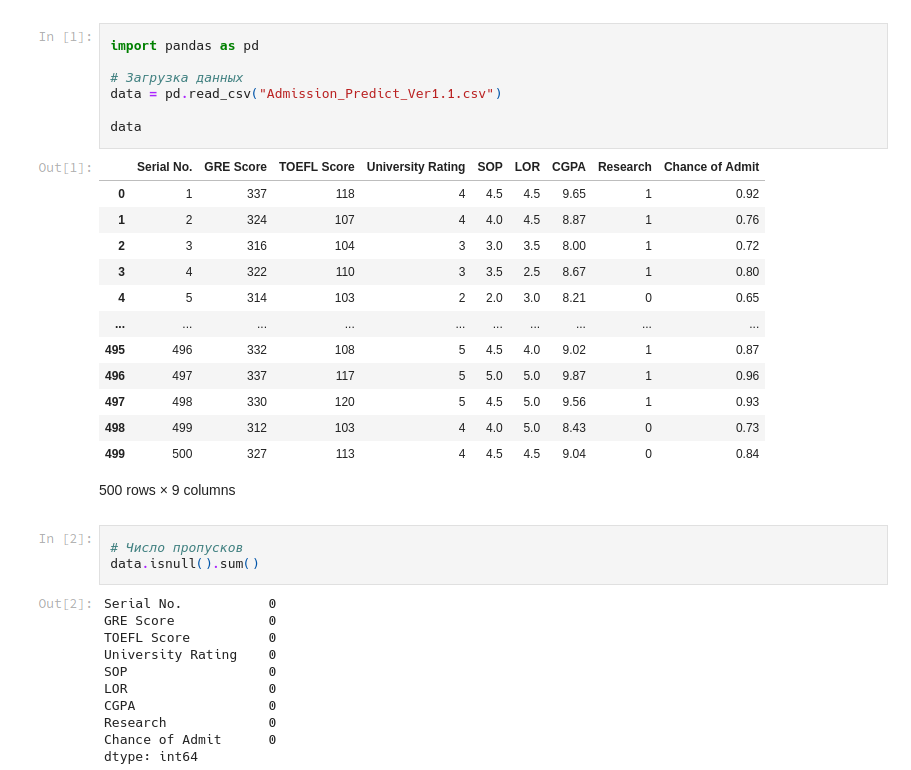
\includegraphics[scale=0.4]{11}
  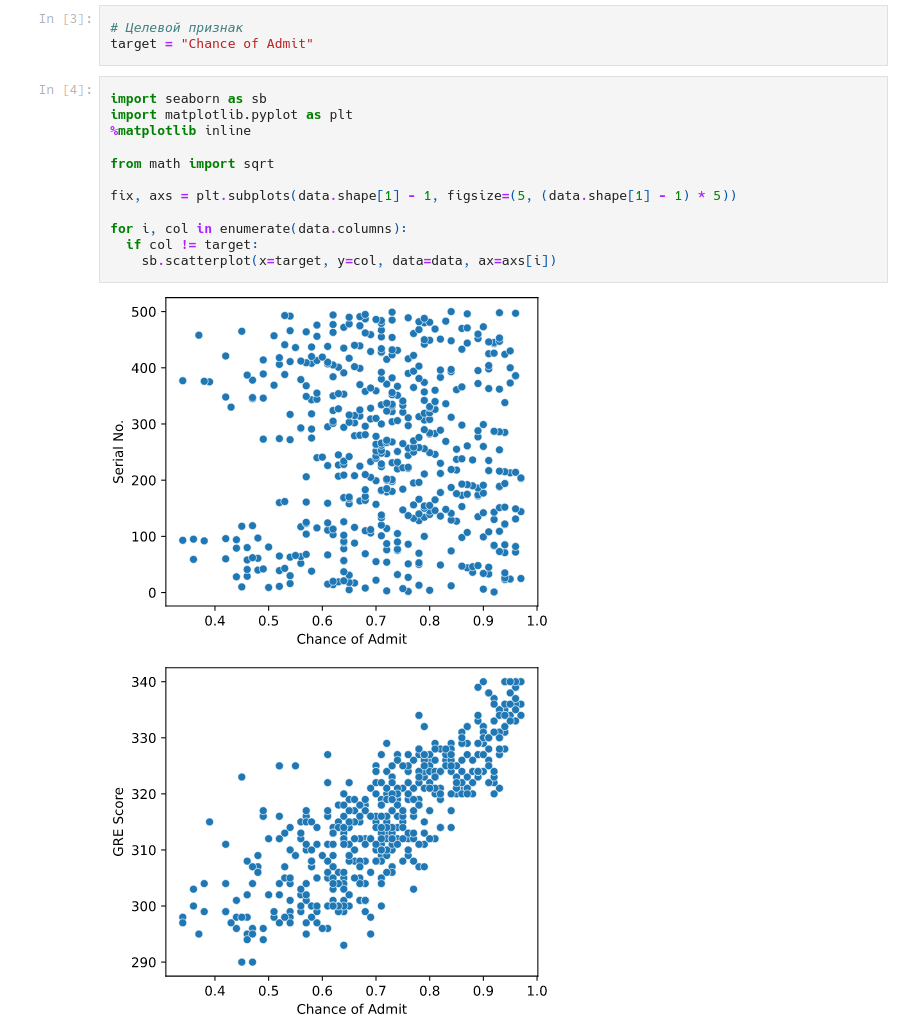
\includegraphics[scale=0.4]{22}
  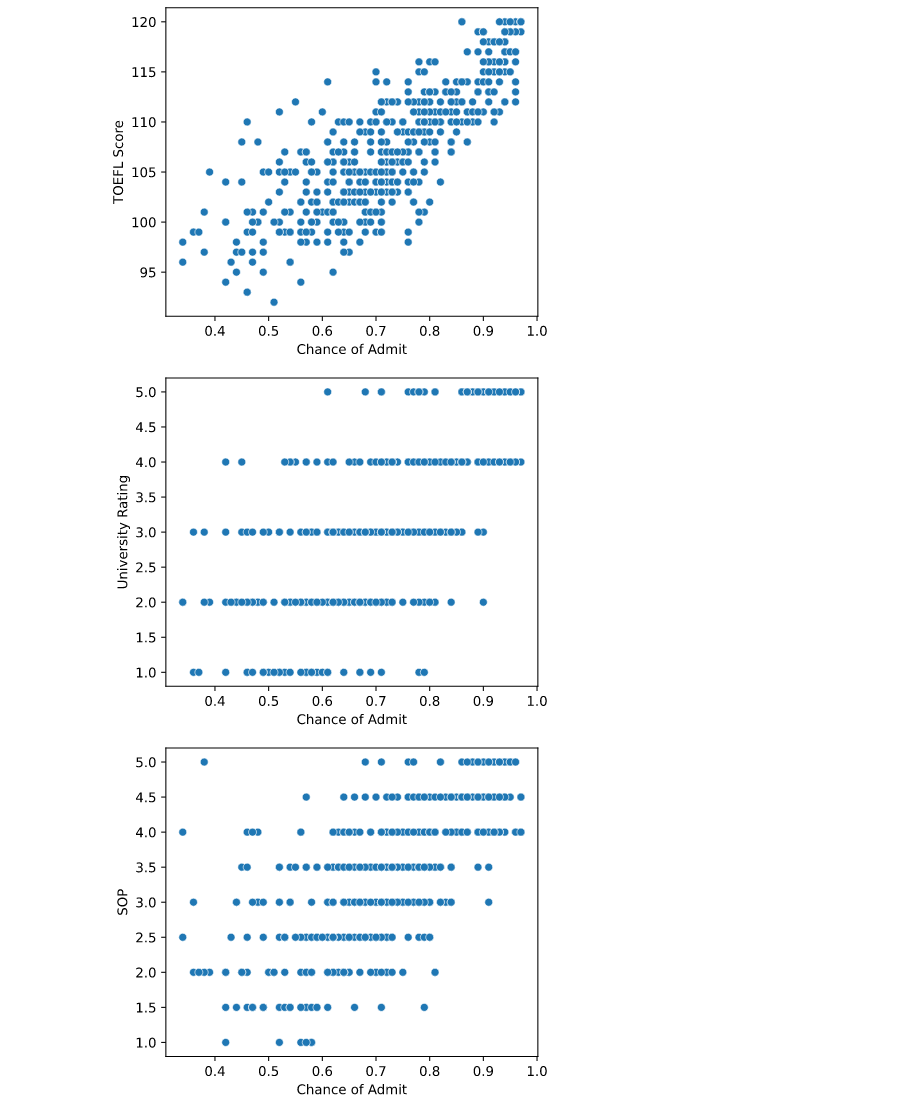
\includegraphics[scale=0.4]{33}
  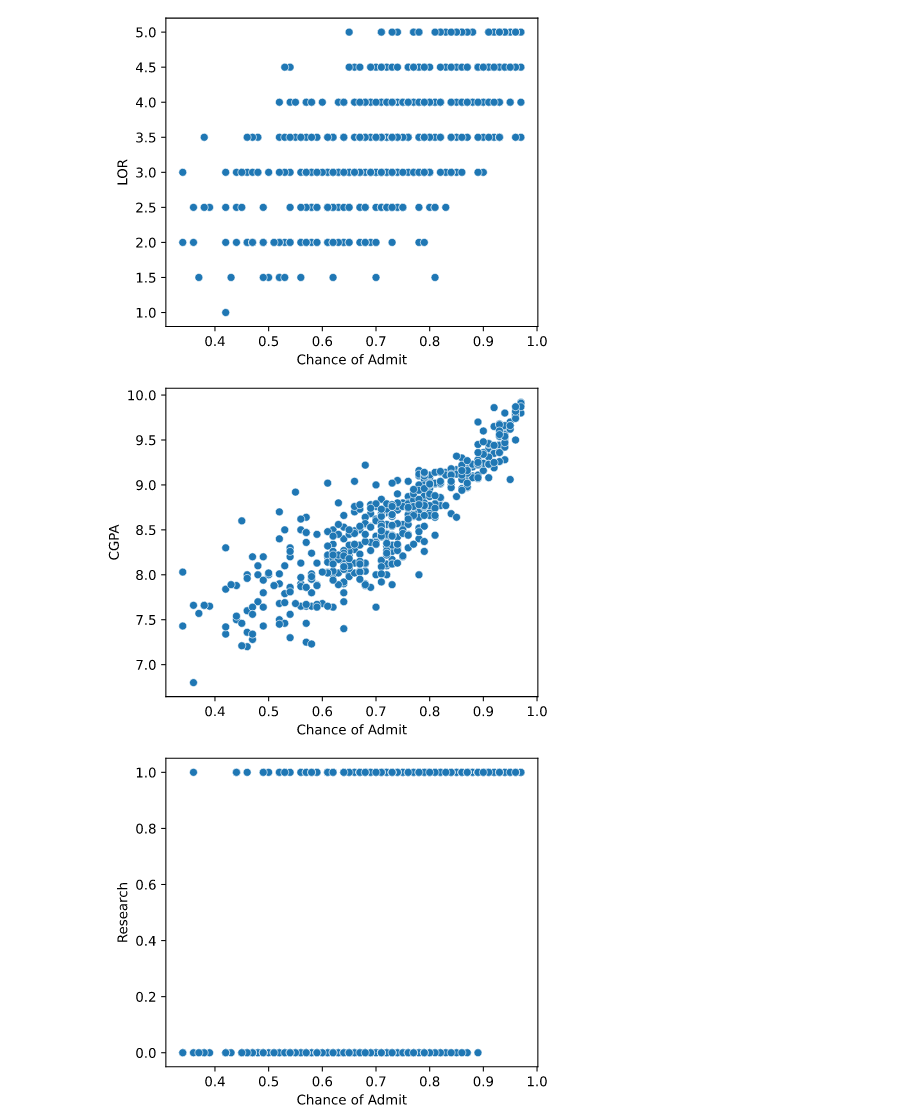
\includegraphics[scale=0.4]{44}
  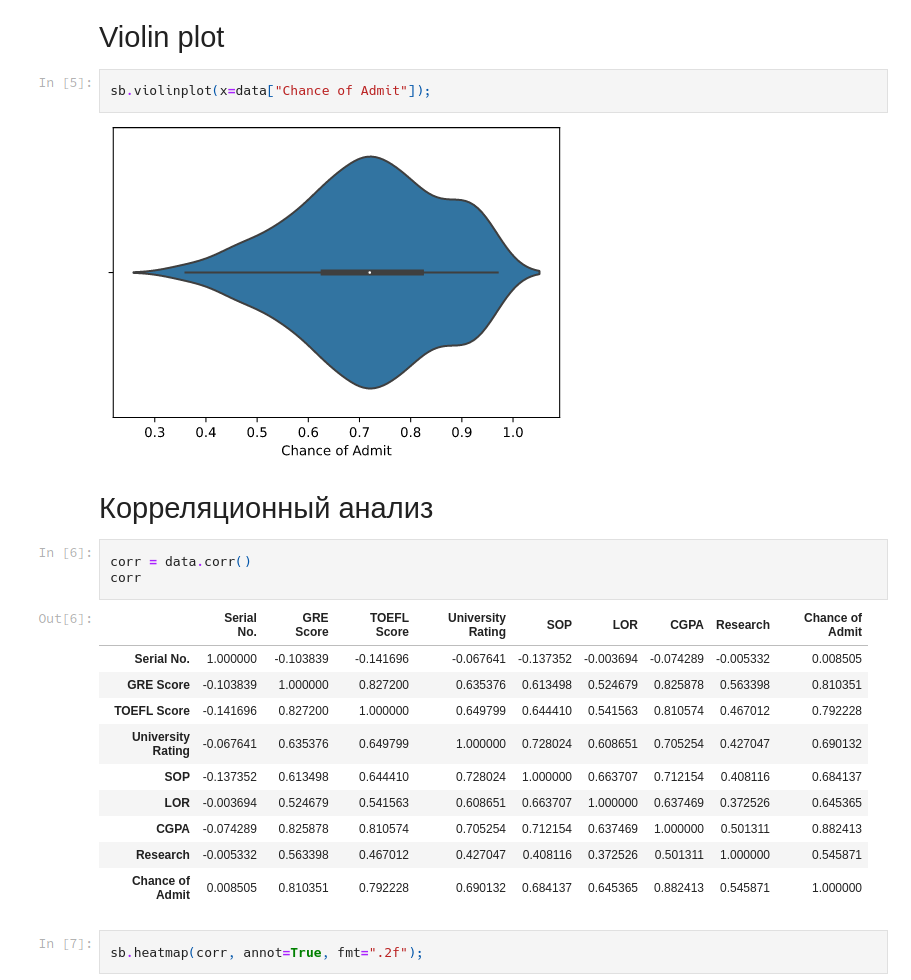
\includegraphics[scale=0.4]{55}
  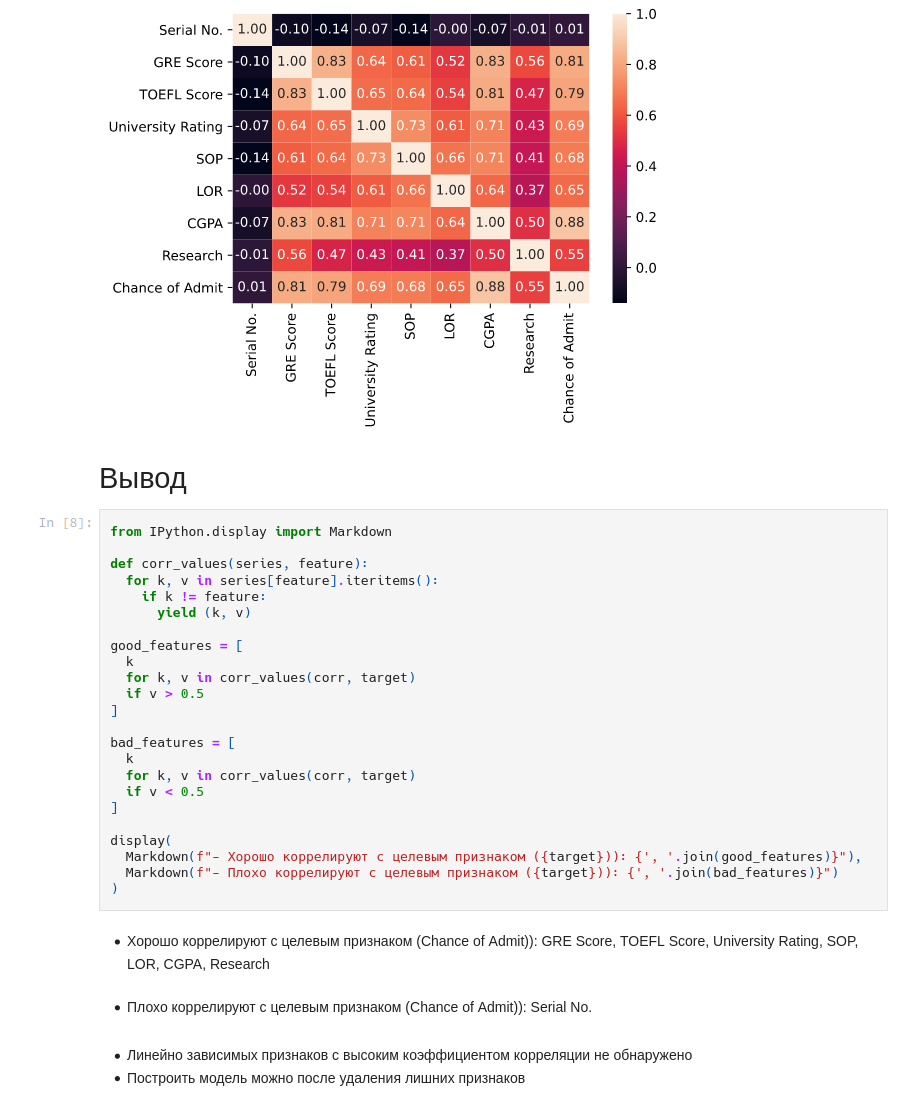
\includegraphics[scale=0.4]{66}
\end{document}
